\chapter{主張}\label{chapter:Prepare}
\section{章の概略}\label{section:Outline}
この章では準備としてペンシルパズルに関わる用語の定義を行う. ただし, ペンシルパズルとは「サイズ$m\times n$の平面グリッドに完成形の条件を明示した問題を与えたとき, 論理的推測から問題を解く行為と, その問題やルールなどを一括りに呼ぶ概念」とし, 明確な定義は行わずあくまで概念として以下もペンシルパズルという用語を使用する.
ペンシルパズルは, 例としてナンバープレイス(\cref{figure:SamplePuzzle})などが与えられる.

\cref{section:WordDefinition}ではペンシルパズルで与えられる盤面と, それに付随する用語を定義する.
\cref{section:MathematicalDefinition}ではペンシルパズルにおける, 諸概念の数学的な定義を行う.
\cref{section:PuzzleRuleDefinition}では\cref{section:MathematicalDefinition}で定義する\textit{codomain}, \textit{conditions}, HI, \textit{identification}という四つの用語を用いて, パズルルールの定義を行う.
\cref{section:Replace}では, \cref{section:MathematicalDefinition}において定義する盤面を変換するシフトという概念の定義を行う.
\cref{section:ConcreteConditions}では\cref{section:MathematicalDefinition}で定義する\textit{conditions}の具体的な構成方法についての説明を行う.

\section{用語の定義}\label{section:WordDefinition}
\cref{section:WordDefinition}では以降の章における理解を助けるためにペンシルパズルにおける位置, 状態, 盤面, 完成盤面, 完成可能盤面という用語を簡単に定義する. \cref{figure:Board}で与えたようなグリッドに対し, 格子点, 細胞, 辺を\textbf{位置}と呼ぶこととする. ただし, 格子点, 細胞, 辺は\cref{figure:Board}で与える図中の名称とそれぞれ対応させるものとする. ペンシルパズルにおいて, その位置に与えられる状態のことを本研究ではそのまま\textbf{状態}と呼ぶこととする. 状態とは, 各位置に対応する写像で送ったその値のことを指すものとする. ソルバーに対し状態が明示されていることを\textbf{既知}, されていないことを\textbf{未知}と呼ぶこととする. 既知である状態のとき, その値を\textbf{解}と呼び, 具体的に数値や定数で与えられるものとする(e.g. 3や$x_1$. ). 未知である状態のとき, その値を特に\textbf{\textit{null}}と表現することとする. さらに, グリッドにおける各格子点, 細胞, 辺全てに状態が存在するときに限り, その状態全体を\textbf{盤面}と定義する. しかし, その状態が未知, 既知に関わらず盤面と呼ぶことに注意する. \cref{figure:SamplePuzzle}に与えたパズルでは, 左上端の細胞の状態が既知であり, その解は2に対応し, 右下端の細胞の状態は未知である(既知の場合解は3).
% TODO: 文献挿入

ここでパズルルールを既存のパズルルールと相違ない定義を行うためにパズルルールにて満たされるべき条件を定義する. 既存のパズルルールにおいてあるパズルルールの問題が存在したとき, それが唯一解であることが条件として参考文献にある. 具体的なパズルルールにおいても唯一解であることが条件として参考文献で確認されている. そのため, 本研究においてもパズルの問題, と呼んだときはそれが唯一解であることを要求することとする. ただしここで呼ぶ唯一解とは, 先の解とは意味が異なり, 問題を解いたとき盤面として答えが一つに定まるそのことを\textbf{唯一解}と呼ぶことに注意する.
以上のことを踏まえ, 全ての格子点, 細胞, 辺の解がパズルルールに定められた条件(\textit{conditions})を満たしている盤面のことを\textbf{完成盤面}と定義する. ある盤面が存在して, 全ての位置の状態が既知であるときにその解が, パズルルールに定められた条件(\textit{conditions})に従う完成盤面がただ一つしかない盤面を\textbf{完成可能盤面}と定義する. 以上の記述より, ある完成盤面もまた完成可能盤面である. 完成可能盤面と完成盤面の例として\cref{figure:SamplePuzzle}を与える. 図中左が完成可能盤面, 図中右が完成盤面である.

上の記述より, 一つの完成盤面には複数の完成可能盤面が対応する(一つの操作(状態が未知である位置に対し具体的な解を対応させること)を課した完成可能盤面もまた完成可能盤面. ). このとき, 一つの完成盤面に対応している完成可能盤面の集合全体をパズルルールの\textbf{問題}と定義する. ある問題に含まれる完成可能盤面を, その完成可能盤面に対応する完成盤面へと変換するその操作のことを問題を\textbf{解く}と呼ぶこととする.
以上のような定義を行うことで問題が唯一解であることを保証する.

\section{盤面に関する数学的定義}\label{section:MathematicalDefinition}
\cref{section:MathematicalDefinition}では\cref{section:WordDefinition}で与えた用語を数学的に定義する. ここで定義するものは全て直感的な定義と違わないように行う.
まず, 平面グリッドを与えたとき, ペンシルパズルの盤面には左上から各格子点に対し座標$(i,j)$を割り振ることができる(\cref{figure:Coordinate}). そうしたとき, グリッドにおける格子点, 細胞, 辺に対して\cref{figure:VariableAtBoard}で表されるように変数を与えることができる.
これをそれぞれ数学的に格子点$p(i,j)$, 細胞$c(i,j)$, 横辺$h(i,j)$, 縦辺$v(i,j)$として定義する.

\begin{definition}[格子点$p(i,j)$, 細胞$c(i,j)$, 横辺$h(i,j)$, 縦辺$v(i,j)$, 位置]\label{definition:VariableAtBoard}
  \textbf{格子点}$p(i,j)$($(i,j)\in \mathbb{N}^2$)を
  \begin{equation}
    p(i,j)\coloneqq \{\,(i,j)\,\} \quad (1\le i \le m+1, 1\le j \le n+1)
  \end{equation}
  と定義する. 以下同様に\textbf{細胞}$c(i,j)$, \textbf{横辺}$h(i,j)$, \textbf{縦辺}$v(i,j)$を
  \begin{align}
     & c(i,j)\coloneqq  \{\,(i,j), (i,j+1), (i+1,j), (i+1,j+1)\,\}  \quad & (1\le i \le m, 1\le j \le n)   \\
     & h(i,j)\coloneqq  \{\,(i,j), (i,j+1)\,\}                      \quad & (1\le i \le m, 1\le j \le n+1) \\
     & v(i,j)\coloneqq  \{\,(i,j), (i+1,j)\,\}                      \quad & (1\le i \le m+1, 1\le j \le n)
  \end{align}
  と定義する. ただし, $h(i,j)$, $v(i,j)$の詳細に興味がない場合は, 任意の辺という意味で辺$e(i_y,j_y,y)$を$e(i_y,j_y,y) \in \{\,h(i_h,j_h), v(i_v,j_v)\,\} \quad (y \in \{\,h,v\,\})$として定義する.   ただし, $y=h$のとき$e(i_h,j_h,h)$は横辺$h(i_h,j_h)$, $y=v$のとき$e(i_v,j_v,v)$は縦辺$v(i_v,j_v)$を指すものとする. $(i_y,j_y)$の範囲は$y$によって指定されるそれぞれの変数によって定義されるものとする($y=h$のときは$1\le i_h \le m-1$, $1\le j_h \le n$).

  また, 格子点, 細胞, 辺の集合の詳細そのものに興味がない場合は任意の格子点, 細胞, 辺という意味で位置$\lambda(i_y,j_y,y)$を$\lambda(i_y,j_y,y) \coloneqq \{\,p(i_p,j_p),c(i_c,j_c),h(i_h,j_h),v(i_v,j_v)\,\} \quad (y \in \{\,p,c,h,v\,\})$と定義する. ただし, $y=p$のときは$\lambda(i_p,j_p,p)$は格子点$p(i_p,j_p$), $y=c$のときは$\lambda(i_c,j_c,c)$は細胞$c(i_c,j_c)$, $y=h$のときは$\lambda(i,j,h)$は横辺$h(i_h,j_h)$, $y=v$のときは$\lambda(i,j,v)$は縦辺$v(i_v,j_v)$を指すものとする. $(i_y,j_y)$の範囲は$y$によって指定されるそれぞれの変数によって定義されるものとする($y=p$のときは$1\le i_p \le m$, $1\le j_p \le n$).
  これら添え字付きの変数を改めて格子点, 細胞, 辺と呼び, これらをまとめた総称として\textbf{位置}と呼ぶこととする.
\end{definition}
ペンシルパズルにおいて, 位置には状態が存在し, これをそのまま\textbf{状態}と定義する. ソルバーにある特定の位置に対し状態が明示されているそのことを\textbf{既知}と呼び, その具体的な数値や定数を\textbf{解}と呼ぶ(e.g. 3や$x_1$. ). しかし特別に辺に関しては「書かれている」ときは1, 「書かれていない」ときは0に対応させるものとする (参照:\cref{definition:Identification}). また, 解として「状態を持たない」ということを明示する場合の定数を特別に$\emptyset$と表現する. 状態が明示されていないことを\textbf{未知}と呼び, そのときの値を特別に\textbf{\textit{null}}と表現する.
以上から, パズルルールを定義するためには状態がどのような集合の元であるかを定義する必要がある. そのために以下で\textit{codomain}という用語を用いて状態の集合を定義する.

\begin{definition}[\textit{codomain}]\label{definition:Codomain}
  位置に対応する状態がとりうる集合のことを\textbf{\textit{codomain}}と定義する. 格子点, 細胞, 辺の\textit{codomain}を表す集合としてそれぞれ$\mathbb{P}$, $\mathbb{C}$, $\mathbb{H}$, $\mathbb{V}$を用いる. $\mathbb{H}$, $\mathbb{V}$の\textit{codomain}が一致している場合にはまとめて$\mathbb{E}$と記述する. \textit{codomain}の詳細に興味がなく, \textit{codomain}全体を考えるときにはそれら集合を含意するものとして$\Lambda$を使用する.
\end{definition}

ここで, 位置が既知であるとき, それぞれの位置には解として具体的な値(1や3などの数値, あるいは$x_1$などの記号)が対応するがその解は列をなしていて同一の値が含んだ列となることがある.
よって\textit{codomain}と解の列は同一視できないことに注意する. また, パズルルールによっては格子点, 細胞, 辺のいずれかに全ての$(i,j)$において状態を持たない場合があり, そのときに限っては\textit{codomain}は$\emptyset$と記述し, 位置に対応する状態が存在しないことを表すこととする. これは$\mathbb{P}=\{\,\emptyset\,\}$と$\mathbb{P}=\emptyset$は同義である. 以下に\textit{codomain}の例を挙げる. 例としては既存のパズルルールのスリザーリンクを用いる. ただし, スリザーリンクのパズルルールは以下のものである(\cite{web:SlitherLink}).
\begin{example}[スリザーリンクのパズルルール]\label{example:SlitherLinkRule}\textup{}
  \begin{enumerate}
    \item 点と点の間にタテヨコに線を引き, 全体で1つの輪っかを作りましょう.\label{SlitherLinkRule_1}
    \item 4つの点で作られた正方形の中にある数字は, その正方形の辺に引く線の数を表しています. 数字のない正方形には, 何本の線を引くかわかりません.\label{SlitherLinkRule_2}
    \item 線を交差させたり, 枝分かれさせたりしてはいけません.\label{SlitherLinkRule_3}
  \end{enumerate}
\end{example}

\begin{example}[スリザーリンクの\textit{codomain}]\label{example:SlitherLinkCodomain}
  スリザーリンクにおいては, \textit{codomain}は以下のように表すことができる.
  \begin{align}
     & \mathbb{P}  =  \emptyset                       \\
     & \mathbb{C}  =  \{\,\textit{null},0,1,2,3,4\,\} \\
     & \mathbb{E}  =  \{\,\textit{null},0,1\,\}
  \end{align}
\end{example}

以上のように\textit{codomain}を考えることにより, 位置が含まれる各集合から, \textit{codomain}に送る写像を考えることができる.
\begin{definition}[写像$\bm{p}$, $\bm{c}$, $\bm{h}$, $\bm{v}$]\label{definition:Mapping}
  格子点$p(i,j)$を過不足なくふくむ集合$\{\,p(i,j)\,\}$から$\mathbb{P}$に送る写像$\bm{p}$を
  \begin{equation}
    \begin{array}{rccc}
      \bm{p}\colon & \{\,p(i,j)\,\} & \longrightarrow & \mathbb{P} \\
                   & p(i,j)         & \longmapsto     & p_{i,j}
    \end{array}
  \end{equation}
  と定義し, $p_{i,j}$を格子点$p(i,j)$の状態$p_{i,j}$と呼ぶこととする.
  以下同様に$\bm{c}$, $\bm{h}$, $\bm{v}$を

  \begin{equation}
    \begin{array}{rccc}
      \bm{c}\colon & \{\,c(i,j)\,\} & \longrightarrow & \mathbb{C} \\
                   & c(i,j)         & \longmapsto     & c_{i,j}
    \end{array}
  \end{equation}
  \begin{equation}
    \begin{array}{rccc}
      \bm{h}\colon & \{\,h(i,j)\,\} & \longrightarrow & \mathbb{H} \\
                   & h(i,j)         & \longmapsto     & h_{i,j}
    \end{array}
  \end{equation}
  \begin{equation}
    \begin{array}{rccc}
      \bm{v}\colon & \{\,v(i,j)\,\} & \longrightarrow & \mathbb{V} \\
                   & v(i,j)         & \longmapsto     & v_{i,j}
    \end{array}
  \end{equation}
  と定義し, それぞれ状態$c_{i,j}$, $h_{i,j}$, $v_{i,j}$と呼ぶこととする.

  ただし, $\bm{h},\bm{v}$の詳細に興味がない場合は, 同様に
  \begin{equation}
    \begin{array}{rccc}
      \bm{e}\colon & \{\,e(i_y,j_y,y)\,\} & \longrightarrow & \mathbb{E}    \\
                   & e(i_y,j_y,y)         & \longmapsto     & e_{i_y,j_y,y}
    \end{array}
  \end{equation}
  と記述する. 上記の写像の詳細に興味がない場合それらの写像全てを含意するものとして$\bm{\lambda}$を用いて
  \begin{equation}
    \begin{array}{rccc}
      \bm{\lambda}\colon & \{\,\lambda(i_y,j_y,y)\,\} & \longrightarrow & \Lambda             \\
                         & \lambda(i_y,j_y,y)         & \longmapsto     & \lambda_{i_y,j_y,y}
    \end{array}
  \end{equation}
  と記述する. 上と同様に状態$e_{i_y,j_y,y}$, $\lambda_{i_y,j_y,y}$と呼ぶこととする.
\end{definition}
集合論の用語を用いると, 状態の列$(\lambda_{1_{y(1,1)},1_{y(1,1)},y_{(1,1)}}, \lambda_{1_{y(1,2)},2_{y(1,2)},y_{(1,2)}},\ldots)$と写像\\
$\bm{\lambda}\colon \{\,\lambda(i_y,j_y,y)\,\} \longrightarrow \Lambda$の間には$\bm{\lambda}(\lambda(i_y,j_y,y))=\lambda_{i_y,j_y,y}$という自然な一対一対応が存在する.
ここで$\{\,\lambda_{i_y,j_y,y}\,\}$は$\{\,\lambda_{1_{y(1,1)},1_{y(1,1)},y_{(1,1)}}, \lambda_{1_{y(1,2)},2_{y(1,2)},y_{(1,2)}},\ldots\,\}$であり, 写像$\bm{\lambda}$は$\{\,\lambda(i_y,j_y,y)\,\}$によって添え字付けられた族である. またこのとき, $\{\,\lambda(i_y,j_y,y)\,\}$は添字集合で, 位置$\lambda(i_y,j_y,y)$はこの写像の添字である.

状態が既知である位置とその解との対応は\cref{definition:Mapping}のように添字によってラベル付けされ, 解同士の関係は\cref{definition:Codomain}直後で記述したように実際に取る値の如何に関わらず別物として扱う.
位置と, その解\cref{definition:Mapping}との対応が全て分かっているとき, 写像はそれらの取る値を全て列として記述すれば$\bm{\lambda}\Leftrightarrow \{\,\lambda_{i_y,j_y,y}\,\}$と同一視することができる.

このような種々の定義を導入することにより, サイズ$m$, $n$と$\mathbb{P}$, $\mathbb{C}$, $\mathbb{E}$を与えたとき任意の盤面を位置とその状態の対応によって定義することができる.
\begin{definition}[盤面\textit{B}]\label{definition:B}
  \textbf{盤面\textit{B}}を以下のように定義する.
  \begin{equation}
    B\coloneqq \{\,\bm{p},\bm{c},\bm{e}\,\}=\Bigl\{\,\{\,p_{i,j}\,\},\{\,c_{i,j}\,\},\{\,e_{i_y,j_y,y}\,\}\,\Bigr\}
  \end{equation}
\end{definition}

ここで, 位置$\lambda(i_y,j_y,y)$が状態$\lambda_{i_y,j_y,y}$と一対一対応することより誤解の恐れがない場合は$\lambda(i_y,j_y,y) \in B  $, $\lambda_{i_y,j_y,y}\in B $と記述する.
このときは$B$は集合として$B=\{\,\lambda(i_y,j_y,y)\,\}$を考え, 状態$\lambda_{i_y,j_y,y}$も$\bm{\lambda}$によりBの元として扱うこととする.
ただし前と同様$\{\,\lambda(i_y,j_y,y)\,\}$とは$\{\,\lambda(1,1,y_{(1,1)}), \lambda(1,2,y_{(1,2)}),\ldots\,\}$を指すものとする.



ここで, 完成盤面, 完成可能盤面, 問題の定義を再度行う(\cref{section:WordDefinition}). ただし, 完成盤面は全ての位置の状態が既知であることを必要条件としている. よって以下で使用する\textit{conditions}には\textit{null}を認めたものがないことが前提にあることに注意する.
\begin{definition}[完成盤面と\textit{conditions}]\label{definition:Conditions}
  全ての位置の状態が既知である盤面を与えたとき, 解が満たしているべき条件を\textbf{\textit{conditions}}と呼ぶ. そしてこれが条件として記述される盤面の集合の任意の元を\textbf{完成盤面}と定義する.
\end{definition}

\begin{definition}[完成可能盤面]
  ある盤面が存在して, 全ての位置の状態が既知としたとき, その解が全て\textit{conditions}に従う完成盤面がただ一つしかないとき, その盤面を\textbf{完成可能盤面}と定義する.
\end{definition}

\begin{definition}[問題]
  一つの完成盤面に対応する完成可能盤面全体の集合を一つの\textbf{問題}と定義する. ただし, 問題の集合は要素として2以上であることを要請するものとする. また, 文脈の中で問題の元として特別, 状態が未知であるものを含む盤面を指したいときは\textbf{非完成盤面}と呼ぶこととする.
\end{definition}

ある盤面を与えたとき, それに対応する完成盤面がただ一つであることを\textbf{唯一解}と呼ぶこととする. 問題の集合が要素として2以上であるから, 必ず非完成盤面も問題に含まれることとなる.
以上のような定義を行うことで, 問題は唯一解であることを保証する.

ここで盤面(\cref{definition:B})全体の集合を考えたとき, 以下のように記述される.
\begin{equation}\label{equation:U}
  U=\Bigl\{\,\{\,\bm{p},\bm{c},\bm{e}\,\}_x\,\Bigr\}=\biggl\{\,\Bigl\{\,\{\,p_{i,j}\,\}_x,\{\,c_{i,j}\,\}_x,\{\,e_{i_y,j_y,y}\,\}_x\,\Bigr\}_x\,\biggr\} \quad (1\le x \le |U|)
\end{equation}
これに\textit{conditions}を条件として与えることで完成盤面全体の集合が下式で与えられる.
\begin{equation}\label{equation:X}
  X=\biggl\{\,\Bigl\{\,\{\,p_{ij}\,\}_x,\{\,c_{ij}\,\}_x,\{\,e_{i_y,j_y,y}\,\}_x\,\Bigr\}_x\mid \rm{\textit{conditions}}\,\biggr\}
\end{equation}
このように与えることであるパズルルールが存在したとき, 完成盤面は$X$の元であると言え, ベン図として\cref{figure:VennDiagram}のように記述することができる.

\textit{conditions}の具体例は\cref{section:ConcreteConditions}で, 具体的な構成方法を示したのちに取り上げることとする(\cref{example:SlitherLinkConditions}).



完成盤面から未知の状態が含まれる完成可能盤面を生成するために「ソルバーから解を隠す位置」として\textit{Hidden Information}(HI)を定義する.
ただし, \textbf{隠す}という言葉は\textit{codomain}から\textit{null}を除いた集合$\Lambda'=\Lambda \setminus \textit{null}$から\textit{codomain}への写像$\phi\colon \Lambda' \longrightarrow \Lambda$を解の列に作用させることとして定義する. ただし, 完成盤面から完成可能盤面を生成する具体的な手法については\cref{section:GenericAlgorithm}で取り上げる. ある完成盤面があって具体的にHIを与えた際には写像は具体的に構成することができ, それは\cref{equation:Phi}で取り上げる.

\begin{definition}[\textit{Hidden Information}(HI)]\label{definition:HiddenInformation}
  ある完成盤面があったとき, ソルバーから隠す位置の部分集合を\textbf{\textit{Hidden Information}(HI)}と定義する.
  ただし, その部分集合はパズルルールによってそれが一意に定まるものではなく完成盤面に依存するものとし, パズルルールでは$\{\,c(i,j)\,\}$と$\{\,e(i_y,j_y,y)\,\}$の部分集合といったように隠す集合及び部分集合の情報のみを指定し, 詳細は指定しないものとする.
\end{definition}

具体的な完成盤面を与えた際には具体的なHIを与えられる. そのとき, 写像$\phi$が具体的に構成することができて,
\begin{equation}\label{equation:Phi}
  \phi(\lambda(i_y,j_y,y))=
  \begin{cases}
    {\lambda(i_y,j_y,y) \quad (\lambda(i_y,j_y,y) \not\in \text{HI})} \\
    {\textit{null} \quad (\lambda(i_y,j_y,y) \in \text{HI})}
  \end{cases}
\end{equation}
と記述することができる.

\begin{example}[スリザーリンクのHI]\label{example:SlitherLinkHiddenInformation}
  \begin{align}
     & \{\,c(i,j)\,\}の部分集合  \\
     & \{\,e(i_y,j_y,y)\,\} \\
  \end{align}
\end{example}

\begin{remark}\label{remark:HI}
  ある完成盤面があってHIを具体的に選び, 解を隠した盤面は完成可能盤面とは限らない.
\end{remark}

なぜなら完成盤面から解を隠した盤面は, 全ての位置の状態を既知にしたとき全ての解が\textit{conditions}に従う完成盤面は一つとは限らないためである(元の完成盤面以外に違う完成盤面が\textit{conditions}に従う可能性がある. ). よってそれはあくまで盤面であり完成可能盤面とはならないことに注意する.
\begin{example}
  例としてスリザーリンクの完成盤面から...を選んだものが図であるが, これは完成盤面として図と図が考えられる. よって図は...
\end{example}
以上より完成盤面の存在は問題の存在と同値にならない. しかし, 既存のパズルルールにおいては先行研究\cite{Fujiwara2022}より以下(\cref{theorem:AutoGeneration})が成立することが示されている. ただし既存のパズルルールとは, 先行研究\cite{Fujiwara2022}が想定しているパズルルールの適用範囲内に従う.
\begin{theorem}\label{theorem:AutoGeneration}
  ある完成盤面が存在したとき, その完成盤面から完成可能盤面を任意に生成することができる. つまり, 完成盤面の存在は問題の存在と同値である.
\end{theorem}
\cref{theorem:AutoGeneration}における, 具体的な生成方法については, \cref{section:GenericAlgorithm}で触れる. ただし, 本研究で定義する全てのパズルルールの任意の完成盤面に未知の状態が含まれる完成可能盤面が存在しているわけではないことに注意する.

ここでHIと関連して, パズルルールによっては\textit{null}と, 解のうちのいずれかがソルバーに同一の状態として示される場合がある. 例としてスリザーリンク(\cref{example:SlitherLinkCodomain})においては$e_{i_y,j_y,y} = 0$のときと$e_{i_y,j_y,y}=\textit{null}$のとき, ソルバーに同一の状態として伝えられていた. これらの対応はパズルルールにおいて明示するべきものである. これを\textit{identification}として定義する. ただし, 同一の状態として示されない(\textit{null}という形でソルバーに示される)場合にはこの対応は明示しないものとする.

\begin{definition}[\textit{identification}]\label{definition:Identification}
  \textit{null}と解のいずれかとがソルバーに同一の状態として伝えられるその対応を\textbf{\textit{identification}}として定義する.
  $\lambda_{i_y,j_y,y}=\textit{null}$と解のいずれか$\lambda_{i_y,j_y,y}=x$を同一の状態として示すことを$\lambda\colon\textit{null}\leftrightarrow x$と表記することとする.
  ただし, 同一の状態として示されない(\textit{null}という形で示される)場合には\textit{identification}を明示しないものとする.
\end{definition}

\begin{example}\label{example:SlitherLinkIndentification}
  スリザーリンクにおける\textit{identification}は
  \begin{align}
     & c\colon\textit{null}\leftrightarrow\emptyset \\
     & e\colon\textit{null}\leftrightarrow 0
  \end{align}
  となる.
\end{example}


\section{パズルルールの定義}\label{section:PuzzleRuleDefinition}
\cref{section:MathematicalDefinition}で定義した概念を用いることによってパズルルールを数学的に定義する. パズルルールに必要とされる条件は\cref{section:WordDefinition}より, 問題が一つ以上存在することである. しかし, \cref{theorem:AutoGeneration}より, 完成盤面の存在は問題の存在と同値である. よって以下のようにペンシルパズルのパズルルールを定義することができる.
\begin{definition}[パズルルール]\label{definition:PuzzleRule}
  \textit{codomain}, \textit{conditions}, HI, \textit{identification}をそれぞれ具体的に与えた際に問題が存在するとき, それらの組み合わせを\textbf{パズルルール}と定義する.
\end{definition}
この定義が既存のパズルルールと相違なく定義できていることを確認し, さらに新しくパズルルールが考えられることを\cref{chapter:3}で実証する.

\section{リプレイス
  % , シフト
 }\label{section:Replace}
既存のパズルルールを説明するにあたり, リプレイス
% とシフト
という概念が必要になるので\cref{section:Replace}にて説明を行う. 直感的には, リプレイスはグリッドを格子点の中心を通るように引き直す操作である.
% シフトは盤面に存在する線を, それ自身を包む領域に辺を組み替える操作である.
リプレイスを行うことにより, 「細胞の中に線を引く」といった既存のパズルルールの\textit{conditions}を扱うことができるようになる.
% またシフトを行うことで, 部屋を扱う盤面をグラフとして記述できるようになる.
ただし, 本質的には同値変形であるので新規のパズルルールを考える際には
リプレイス
% とシフト
を行う必要はない.

\cref{figure:Replace}のようにグリッドを引き直す操作を数学的に定義する.
\begin{definition}[リプレイス]\label{definition:Replace}
  盤面$B$を与えられたとき, 以下の変換を考えることができる.
  \begin{align}
    \bm{f_p}\colon & p(i,j)  \longmapsto c'(i,j) \\
    \bm{f_c}\colon & c(i,j)  \longmapsto p'(i,j)
  \end{align}
  ただし, 変換後の座標は左上を$(0,0)$とする.
  また, それぞれの位置に対応する状態も, 変換後の位置に対応させるものとする. 辺$e(i_y,j_y,y)$は$p(i,j)$を繋いでいたものをそのまま$c'(i,j)$を繋ぐものとし, \cref{figure:Replace}のように辺を対応させ, 状態も変化させないものとする. 変換後のグリッド上の見かけの辺には位置, 状態ともに割り当てないものとする.ただし, $p'_{0,n'}$, $p'_{m+1,n'}$, $p'_{m',0}$, $p'_{m',n+1}$はそれぞれ$\emptyset$とする.$(0\le m' \le m+1$, $0\le n'\le n+1)$.

  このような変換をいかなる盤面においても考えることができ, これらの写像$\bm{f_p}$, $\bm{f_c}$をまとめて行う操作のことを\textbf{リプレイス}と定義する.
\end{definition}
上記のリプレイスを用いることで, \textit{conditions}が表現できる既存のパズルルールが存在する. 具体例としては, \cref{section:ExistsPuzzleRule}で取り上げるナンバーリンク等である. 便宜上, リプレイスを行った盤面を\textbf{置換盤面}と以下では呼ぶこととする. 置換盤面が含まれる集合は元の集合\cref{equation:U}ではなく, 辺と格子点を取り替えた集合に含まれることに注意する.


% \cref{definition:B}のような盤面を考えたとき, 盤面の格子点と細胞の役割を入れ替える操作を考えることができる. 具体的な構成方法は後の\cref{definition:Shift}で触れるが, 概略として, 格子点$p(i,j)\mapsto$細胞$c'(i,j)$, 細胞$c(i,j)\mapsto$格子点$p'(i+1,j+1)$へと盤面をそのまま左上に半単位だけ変換することができる. 辺$e(i_y,j_y,y)$に関しては, その辺をまたがないように変換後は辺を構成することで新たに盤面を記述することができる. これらの変換は一対一写像であり, 逆写像も存在することにより同一の盤面として扱うことができる. このような変換を本研究ではシフト, 逆シフトと呼び, これを以下で定義する. ただし, シフト後の盤面は, シフト前の盤面全体集合の元に一般的には含まれないことに注意する.
% \begin{definition}[シフト, 逆シフト]\label{definition:Shift}
%   盤面$B$を与えられたとき, 以下の変換を考えることができる.
%   \begin{align}
%     \bm{f_p}\colon & p(i,j)  \longmapsto c'(i,j)     \\
%     \bm{f_c}\colon & c(i,j)  \longmapsto p'(i+1,j+1)
%   \end{align}
%   それぞれの位置に対応する状態も, 変換後の位置に対応させるものとする. また, 辺に関しても以下の変換を考えることができる.
%   \begin{align}
%     \bm{f_h}\colon & h(i,j)  \longmapsto v'(i,j+1) \\
%     \bm{f_v}\colon & v(i,j)  \longmapsto h'(i+1,j)
%   \end{align}
%   ただし, 辺に関しては状態を反転させるものとする(e.g. $h_{3,4}=1$のとき, $v'_{3,5}=0$). また, $h'_{1,n'}$, $h'_{m+2,n'}$, $v'_{m',1}$, $v'_{m',n+2}$は全て値として1を取り, $p'_{1,n'}$, $p'_{m+2,n'}$, $p'_{m',1}$, $p'_{m',n+2}$はそれぞれ$\emptyset$とする. $(1\le m' \le m+1$, $1\le n'\le n+1)$

%   このような変換をいかなる盤面でも考えることができ, これらの写像$\bm{f_p}$, $\bm{f_c}$, $\bm{f_h}$, $\bm{f_v}$をまとめて行う操作のことを\textbf{シフト}と定義する. これらは一対一写像であるからいつでも逆写像が存在して, その逆写像を\textbf{逆シフト}と定義する.
% \end{definition}
% 上記のシフトを用いることで, ソルバーに分かりやすい情報の提示が可能になる場合がパズルルールによっては存在する. 便宜上, シフトを行った盤面を\textbf{変換盤面}と以下では呼ぶこととする. 変換盤面が含まれる集合は\cref{equation:U}とは異なることに注意する($p'_{1,n'}$, $p'_{m+2,n'}$, $p'_{m',1}$, $p'_{m',n+2}$は状態を考えないため. ).

\section{{\it conditions}の具体的な構成方法}\label{section:ConcreteConditions}
\cref{section:ConcreteConditions}ではパズルルールの特性を左右する\textit{conditions}を具体的に構成する方法について\cref{example:SlitherLinkConditions}や\cref{chapter:3}で登場するもののみについて説明を行う. ただし, ここで触れる構成方法については限定的なものであり他に記述する際には新たな概念を導入する必要がある場合がある. ただし, 本論文の主旨とは少し異なるため詳しくは触れないものとする.
\subsection{関数}\label{subsection:Function}
\textit{conditions}を構成するにあたり, 関数を定義しておくと便利な場合が多い. ここでは, その中でも頻用するcross関数とcycle関数について定義を行っておく.
完成盤面においては位置と解が一対一に対応することにより, $\mathbb{E}$が要素として数値のみを持つ場合に限り新たに下記のような関数を導入することができる(\cref{figure:cross}, \cref{figure:cycle}).

\begin{definition}[\text{cross}, \text{cycle}]\label{definition:Function}
  \begin{align}
    \text{cross}(p(i,j))\coloneqq h_{i,j-1}+v_{i-1,j}+h_{i,j}+v_{i,j} \\
    \text{cycle}(c(i,j))\coloneqq h_{i,j}+v_{i,j}+h_{i+1,j}+v_{i,j+1}
  \end{align}
\end{definition}

直感的にはcross関数はある格子点$p(i,j)$を与えたとき, その格子点を通る辺の本数を返す関数であり, cycle関数はある細胞$c(i,j)$を与えたとき, その細胞をの周りにある辺の本数を返す関数である.
繰り返しになるが, ここで取り上げる関数は\textit{conditions}を記述するにあたり\cref{example:SlitherLinkConditions}や\cref{chapter:3}を含む, 多くのパズルルールで使用されるというものであり他のパズルルールにおいては他の関数が必要になることがあることに注意する.

\subsection{位置の関係性の定義}\label{subsection:RelationDefinition}

次に, \cref{section:MathematicalDefinition}で定義した位置同士の関係性について定義を行う. ただし, ここでは完成盤面を仮定する.
まず, 連結, 含有, 隣接, 到達可能の定義を行う.
直感的には各用語は以下の意味として導入する.
連結とは辺と辺が繋がっていることである.
含有とは位置が集合として他の位置を含むことである.
隣接とは細胞と細胞が辺を共有していることである.
到達可能とは離れた辺と辺へと向かう道が存在することである.

\begin{definition}[連結]\label{definition:Connection}
  辺$e(i_y,j_y,y)$と辺$e(i_{y'}',j_{y'}',y')$が\textbf{連結}であるとは, 以下が成立することで定義する.
  \begin{equation}
    \begin{cases}
      {e_{i_y,j_y,y}=1,\quad e_{i_{y'}',j_{y'}',y'}  =     1          } \\
      {e(i_y,j_y,y)\cap e(i_{y'}',j_{y'}',y')  \neq  \emptyset}
    \end{cases}
  \end{equation}
\end{definition}

\begin{definition}[含有]\label{definition:Contain}
  辺$e(i_y,j_y,y)$が格子点$p(i',j')$を\textbf{含む(含有する)}とは以下が成立することで定義する.
  \begin{equation}
    \begin{cases}
      {e_{i_y,j_y,y}=1               } \\
      {e(i_y,j_y,y)\supset p(i',j')}
    \end{cases}
  \end{equation}
  以下同様に, 細胞$c(i,j)$が辺$e(i_{y'}',j_{y'}',y')$を含む, 細胞$c(i,j)$が格子点$p(i',j')$を含むことを以下が成立することでそれぞれ定義する.
  \begin{equation}
    \begin{cases}
      {e_{i_{y'}',j_{y'}',y'}=1 } \\
      {c(i,j)\supset e(i_{y'}',j_{y'}',y')}
    \end{cases}
  \end{equation}
  \begin{align}
    c(i,j)\supset p(i',j')
  \end{align}
\end{definition}
このような含有の概念を考えることで細胞, 辺が持つ集合を考えることができる. それらを$P_{c(i,j)}$, $E_{c(i,j)}$, $P_{e(i_y,j_y,y)}$として以下で定義する. ただし, $c(i,j)\supset e(i_{y'}',j_{y'}',y')$などと記述する場合には$c(i,j)$に(本研究における)含まれる$e(i_y,j_y,y)$という意味で用いる.
\begin{definition}[$P_{c(i,j)}$, $E_{c(i,j)}$, $P_{e(i_y,j_y,y)}$]
  細胞$c(i,j)$が含む格子点の集合$P_{c(i,j)}$, 細胞$c(i,j)$が含む辺の集合$E_{c(i,j)}$, 辺$e(i_y,j_y,y)$が含む格子点の集合$P_{e(i_y,j_y,y)}$を以下で定義する.
  \begin{align}
    P_{c(i,j)}       & \coloneqq \{\,p(i',j') \mid \forall p(i',j') \subset c(i,j)\,\}                           \\
    E_{c(i,j)}       & \coloneqq \{\,e(i_{y'}',j_{y'}',y') \mid \forall e(i_{y'}',j_{y'}',y') \subset c(i,j)\,\} \\
    P_{e(i_y,j_y,y)} & \coloneqq \{\,p(i',j') \mid \forall p(i',j') \subset e(i_y,j_y,y)\,\}
  \end{align}
\end{definition}


\begin{definition}[隣接]\label{definition:Adjacent}
  細胞$c(i,j)$と細胞$c'(i,j)$が\textbf{隣接する}とは以下が成立することで定義する.
  \begin{equation}
    E_{c(i,j)} \cap E_{c(i',j')} \neq \emptyset
  \end{equation}
\end{definition}


\begin{definition}[到達可能]
  $e(i_y,j_y,y)$と連結な$e(i_{y_1},j_{y_1},y_1)$, $e(i_{y_1},j_{y_1},y_1)$と連結な$e(i_{y_2},j_{y_2},y_2),\ldots,e(i_{y_t},j_{y_t},y_t)$と連結な$e(i_{y'}',j_{y'}',y')$のような集合$\{\,e(i_{y_1},j_{y_1},y_1),e(i_{y_2},j_{y_2},y_2),\\
    \ldots,e(i_{y_t},j_{y_t},y_t)\,\}$がただ一つでも存在するとき, $e(i_y,j_y,y)$から$e(i_{y'}',j_{y'}',y')$に\textbf{辿ることができる(到達可能である)}と定義する. ただし, 自分自身は常に辿ることができるものとする.
\end{definition}

\begin{remark}
  $e(i_y,j_y,y)$から$e(i_{y'}',j_{y'}',y')$に辿ることができる(到達可能である)ときは定義より常に$e(i_{y'}',j_{y'}',y')$から$e(i_y,j_y,y)$に辿ることができる.
\end{remark}

\begin{example}[連結, 含有, 隣接, 到達可能]
  \cref{figure:SamplePuzzle}において, $h(4,1)$と$v(1,4)$は連結であり, $c(3,4)$は$v(4,4)$のみを含み, $c(2,2)$と$c(2,3)$は隣接しており, $h(3,8)$から$v(8,1)$へは辿ることができる.
\end{example}
以上の定義を用いることによって, 新たに「線」という概念を導入することができる.

\begin{definition}[線]\label{definition:Line}
  盤面に存在する全ての辺を含む集合$\{\,e_{i,j}\,\}$の部分集合$L$の全ての要素から任意の2つの元を取り出したとき, いつでもそれらが互いに辿ることができるときその集合$L$を\textbf{線}であると定義する.
\end{definition}
この線はグラフ理論の用語を用いたときの連結グラフとほとんど同義である. \cref{figure:SamplePuzzle}において, 集合$\{\,h(3,2),v(4,1),h(4,1),h(5,1)\,\}$は線である. この線も含有という関係性を定義することができて,
\begin{definition}[線の含有]
  線$L$が線$L'$を含むとは以下が成立することで定義する.
  \begin{equation}
    L\supset L'
  \end{equation}
  同様に線$L$が辺$e(i_y,j_y,y)$, 格子点$p(i,j)$が含むことを以下が成立することでそれぞれ定義する.
  \begin{equation}
    \begin{cases}
      {L\supset  e(i_y,j_y,y) } \\
      {L\ni \exists e(i_y,j_y,y) \quad \mbox{s.t. $e(i_y,j_y,y)$が$p(i,j)$を含む}}
    \end{cases}
  \end{equation}
\end{definition}

\subsection{グラフ}\label{subsection:GraphDefinition}
\cref{subsection:RelationDefinition}で定義した概念を用いることによって, 盤面$B=\Bigl\{\,\{\,p_{i,j}\,\},\{\,c_{i,j}\,\},\{\,e_{i_y,j_y,y}\,\}\,\Bigr\}$を与えたとき, 盤面上にグラフという概念を導入することができる.

\begin{definition}[グラフ]\label{definition:GraphDefinition}
  グラフ$G_z$を以下で定義する.
  \begin{equation}
    G_z=\{\,P_z,L_z\,\}=\biggl\{\, \Bigl\{\,p(i,j)\,\Bigr\}_z,\Bigl\{\,e(i_y,j_y,y)\,\Bigr\}_z\,\biggr\}
  \end{equation}
  ただし, $L_z$はある$e(i_y,j_y,y)$が存在したとき盤面上に存在する$e(i_y,j_y,y)$を含む線の中で集合として最大の線であり, $P_z$は$L_z$が含む全ての$p(i,j)$の和集合とする. ただし, どの線にも含まれない$p(i,j)$もグラフと呼び, そのときに限り$G_z=\{\,p(i,j)\,\}$とし, \textbf{孤立点}と呼ぶこととする($\{\,p(i,j)\,\}$は集合として, 一つの要素$p(i,j)$しか持たない集合).
\end{definition}

このようなグラフという概念が盤面に存在すると考えられ, 盤面上のグラフ全てを要素に持つ集合
\begin{equation}
  A=\{\,G_1,G_2,\ldots,G_a\,\}=\{\,G_z\,\}\quad (aは盤面に存在するグラフの数)\label{equation:A}
\end{equation}
がいつでも一意に定まる. (\cref{section:GraphUnique})

また\cref{definition:Function}で取り上げた関数のうち, グラフが定義に$p(i,j)$を含むことにより$\text{cross}$を用いて「グラフ内の全ての$p(i,j)$において, $\text{cross}(p(i,j))=2$」などという条件を構成できる. グラフという概念を導入したことにより, \cref{definition:Conditions}で取り上げた\textit{conditions}を記述することができる.
\begin{example}\textup{スリザーリンクの\textit{conditions}}\label{example:SlitherLinkConditions}
  スリザーリンクの\textit{conditions}は
  \begin{align}
     & B\ni \forall p(i,j)   , \forall c_{i,j} , \text{cross}(p(i,j))=c_{i,j}\label{equation:SlitherLinkConditions_1} \\
     & G_1\ni \forall p(i,j)            , \text{cross}(p(i,j))=2             \label{equation:SlitherLinkConditions_2} \\
     & G_xは孤立点(x\ge 2)                                                     \label{equation:SlitherLinkConditions_3}
  \end{align}
  となる.
\end{example}

\begin{clearpagefigure}
  
\includegraphics[width=0.8\linewidth,clip]{fig/board.png}
  \caption{}
  \label{figure:Board}
\end{clearpagefigure}

\begin{clearpagefigure}
  
\includegraphics[width=0.8\linewidth,clip]{fig/samplePuzzle.png}
  \caption{サンプルパズル}
  \label{figure:SamplePuzzle}
\end{clearpagefigure}

\begin{clearpagefigure}
  
\includegraphics[width=0.8\linewidth,clip]{fig/coordinate.png}
  \caption{}
  \label{figure:Coordinate}
\end{clearpagefigure}

\begin{clearpagefigure}
  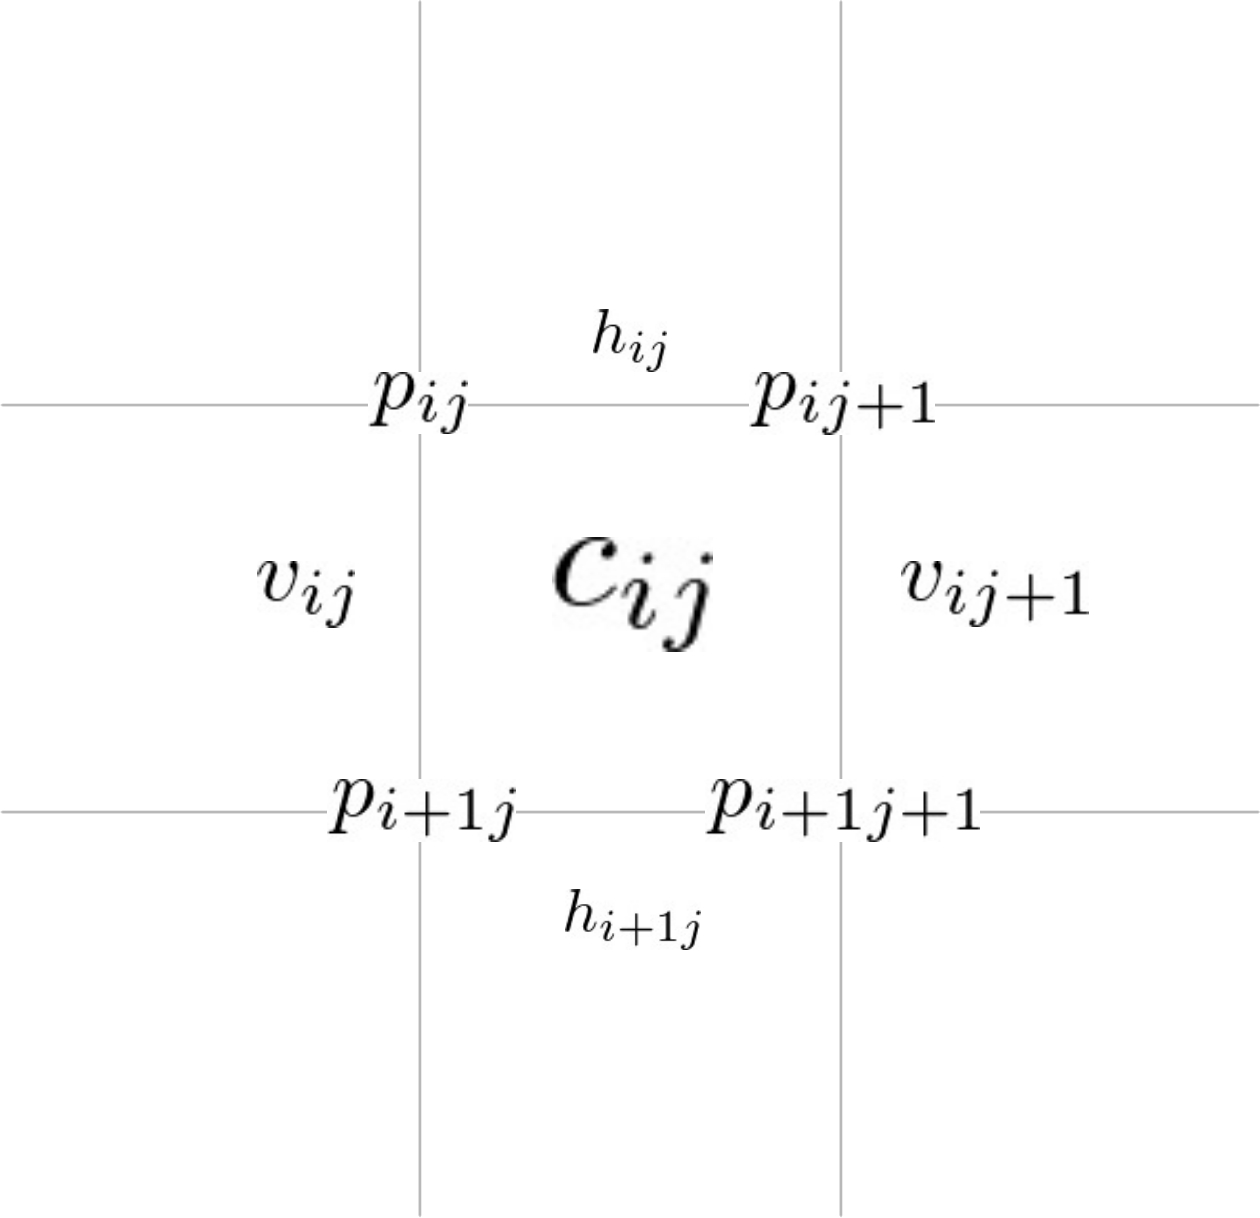
\includegraphics[width=0.8\linewidth,clip]{fig/define.png}
  \caption{}
  \label{figure:VariableAtBoard}
\end{clearpagefigure}

\begin{clearpagefigure}
  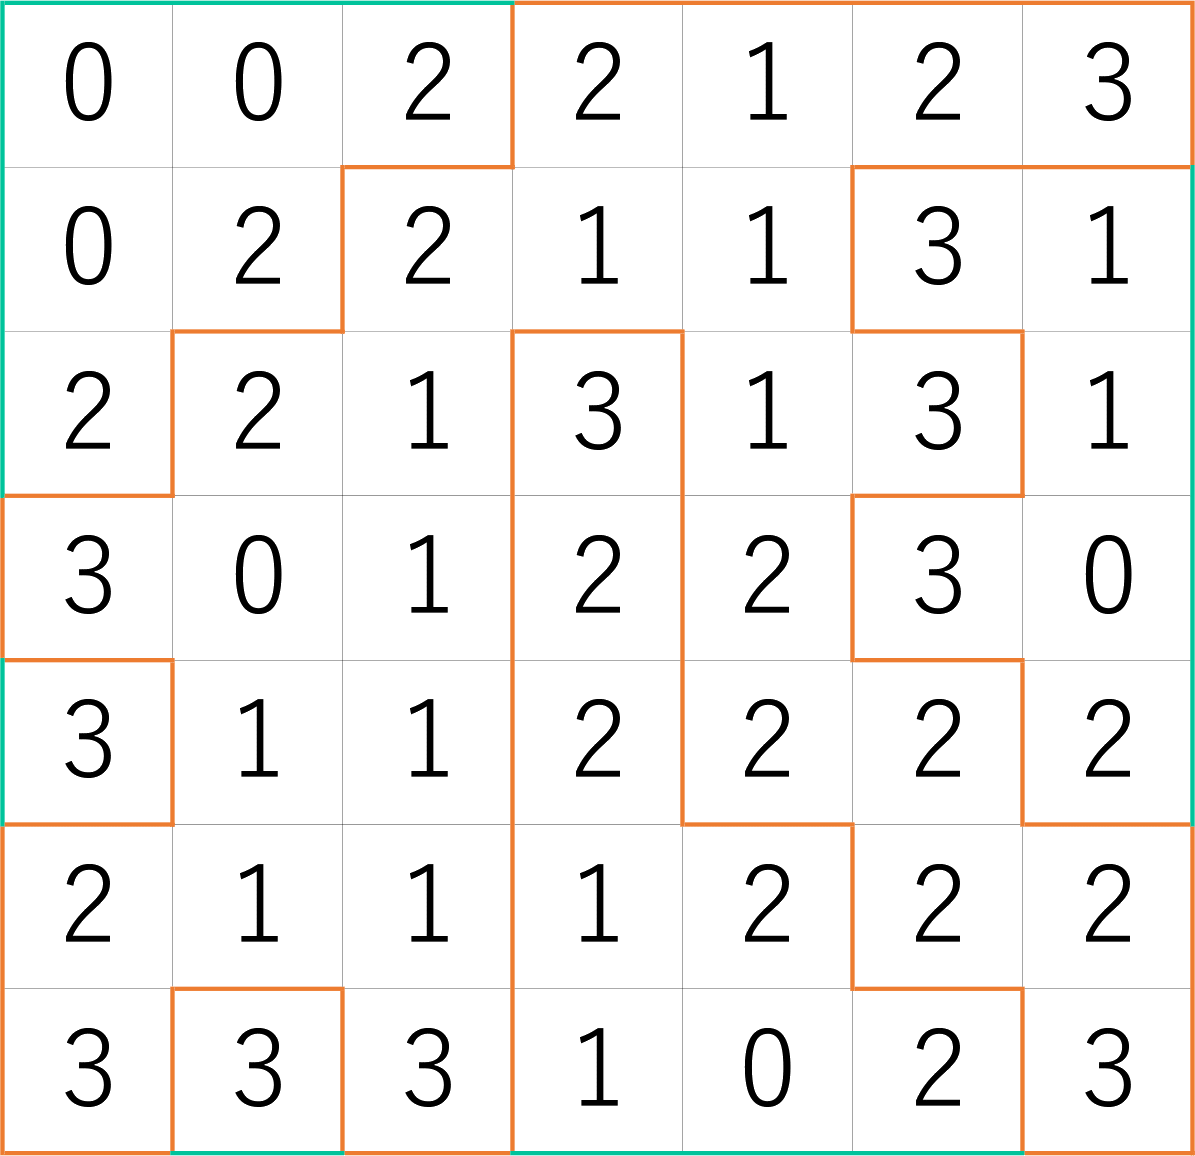
\includegraphics[width=0.8\linewidth,clip]{fig/slitherlink.png}
  \caption{スリザーリンクの完成盤面}
\end{clearpagefigure}

\begin{clearpagefigure}
  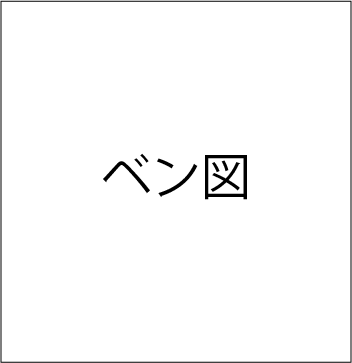
\includegraphics[width=0.8\linewidth,clip]{fig/vennDiagram.png}
  \caption{}
  \label{figure:VennDiagram}
\end{clearpagefigure}

\begin{clearpagefigure}
  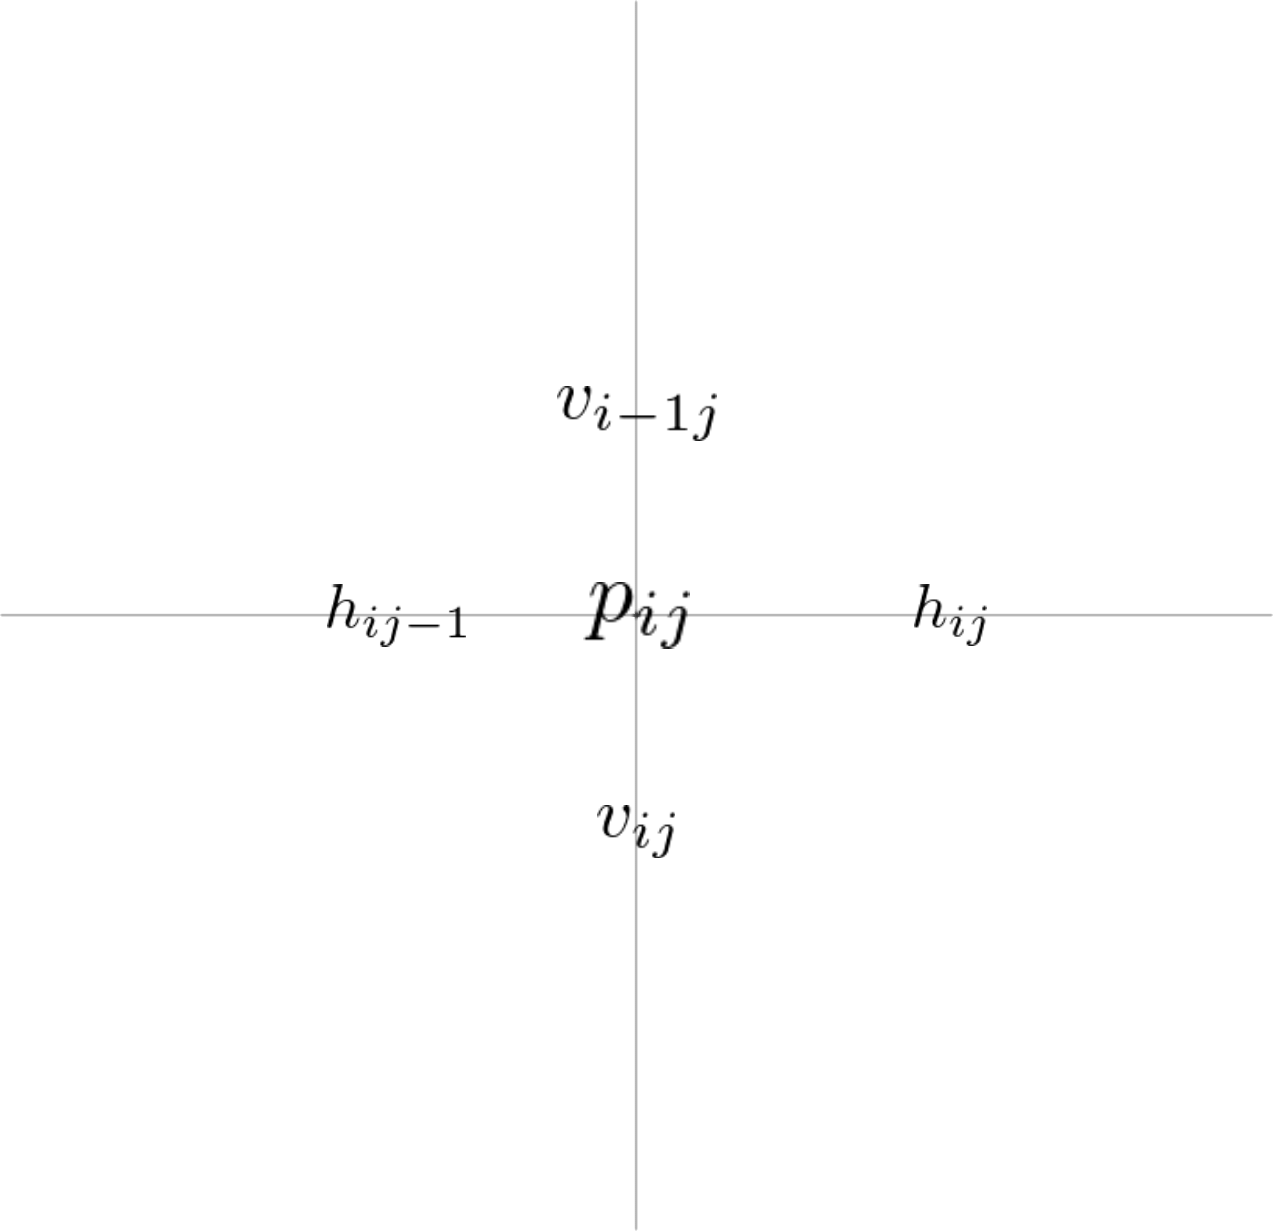
\includegraphics[width=0.8\linewidth,clip]{fig/cross.png}
  \caption{cross}
  \label{figure:cross}
\end{clearpagefigure}

\begin{clearpagefigure}
  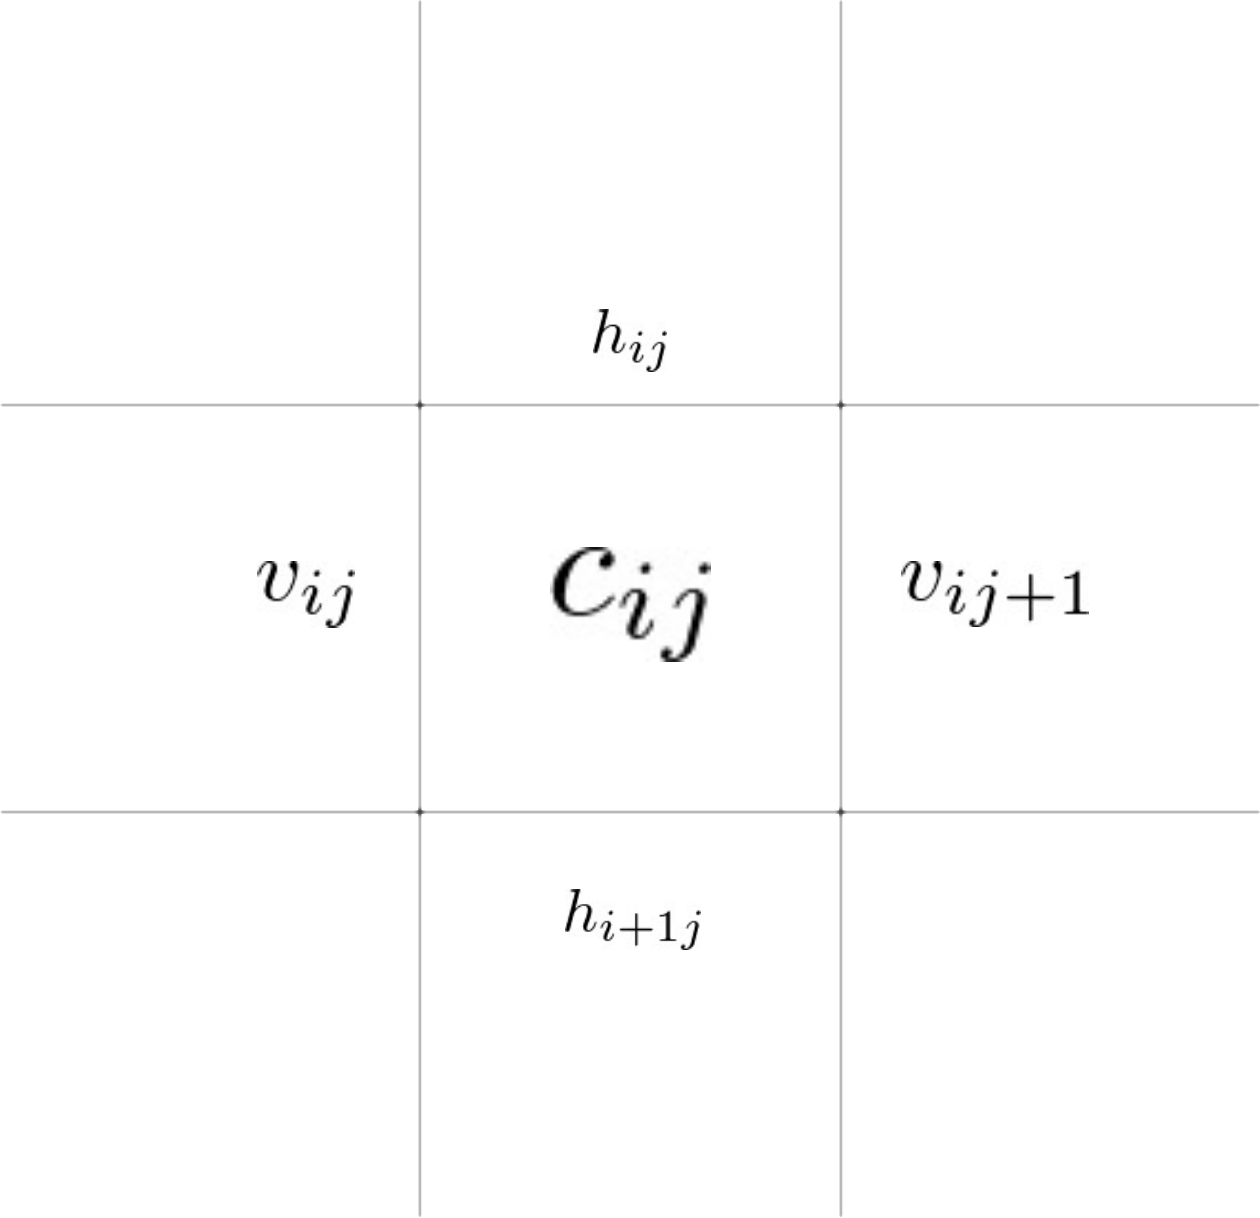
\includegraphics[width=0.8\linewidth,clip]{fig/cycle.png}
  \caption{cycle}
  \label{figure:cycle}
\end{clearpagefigure}

\begin{clearpagefigure}
  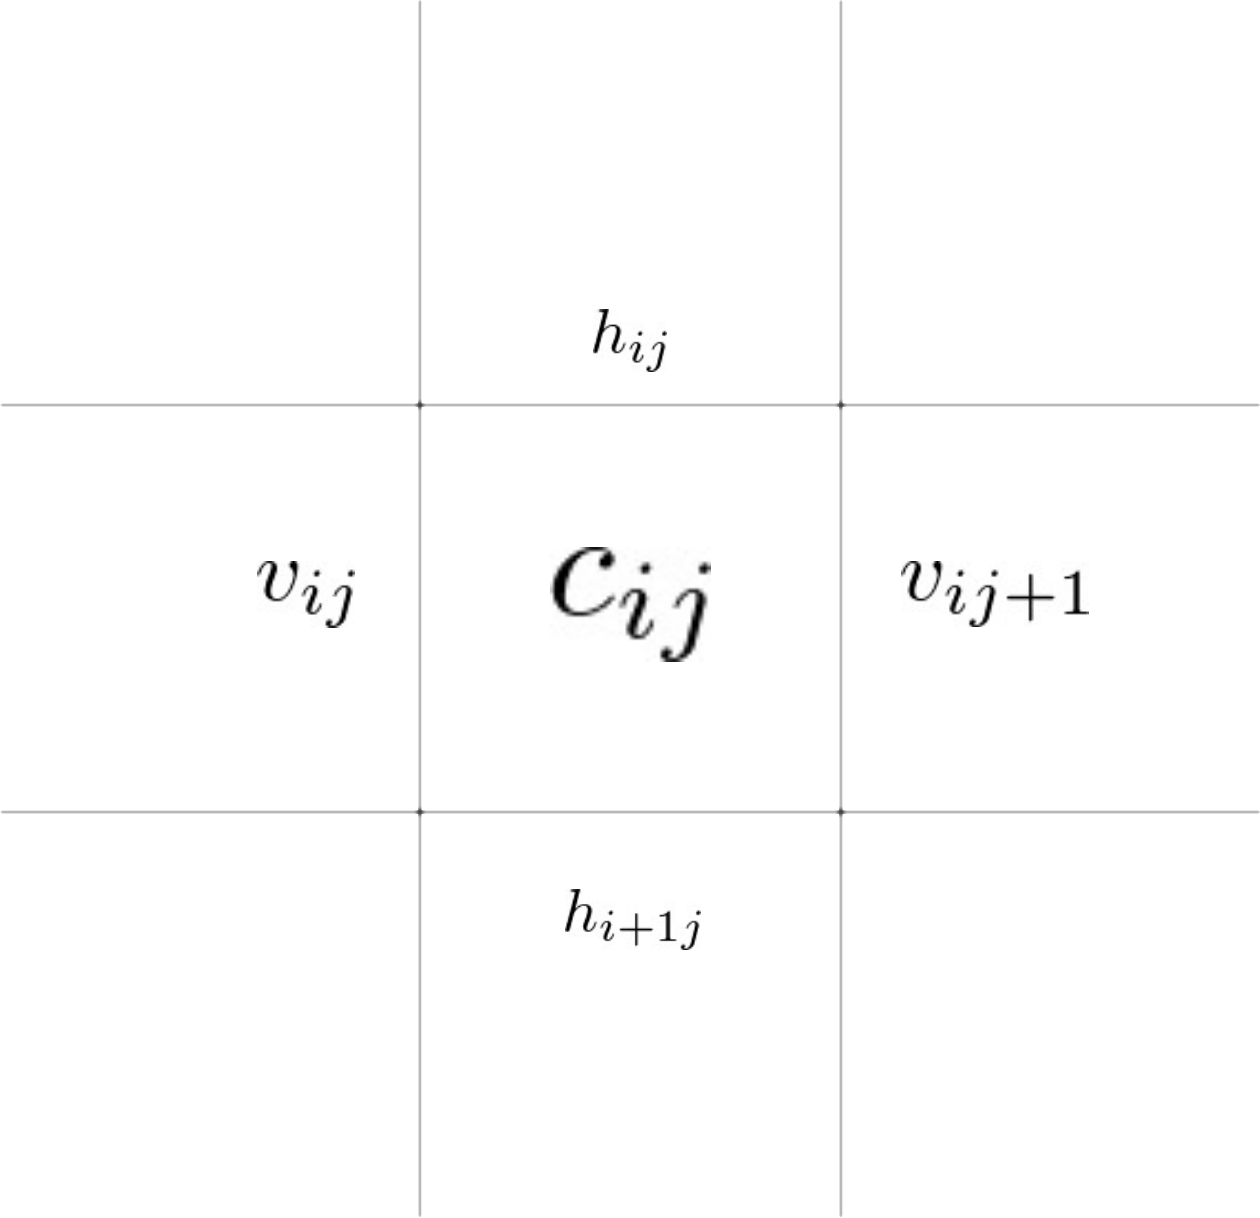
\includegraphics[width=0.8\linewidth,clip]{fig/cycle.png}
  \caption{replace}
  \label{figure:Replace}
\end{clearpagefigure}
